\documentclass{beamer}
\author{\textbf{Benjamin Isenhart}\inst{1},Ekraj Dahal\inst{2}, Karen Cianciulli\inst{3}, Matthew S. White\inst{1}\inst{2}}
\institute[UVM]{\inst{1} Department of Physics, The University of Vermont, Burlington VT\\
\inst{2} Materials Science Pgrogram, The University of Vermont, Burlington VT\\
\inst{3} Asheville School, Asheville NC}
\title{Precise Control of Organic LED Emission Through Optically-Resonant Microcavity Confinement}
\date{May 2, 2019}
%\logo{
\includegraphics[height=1.5cm]{images/uvm_logo_stacked.png}}
\usepackage[utf8]{inputenc}
\usepackage{amsfonts}
\usepackage{amsmath}
\usepackage{physics}
\usepackage{graphicx}
\usepackage{wrapfig}
\usetheme{default}

\begin{document}

\begin{frame}
    \titlepage
\end{frame}
\begin{frame}
    \tableofcontents
\end{frame}

\section{Introduction}
    \frame{\tableofcontents[currentsection]}
    
    \subsection{OLED Devices}
        \begin{frame}
            \frametitle{OLED Devices}
            \begin{columns}
				\begin{column}{0.4\textwidth}
				 
				\end{column}
				\begin{column}{0.6\textwidth}
					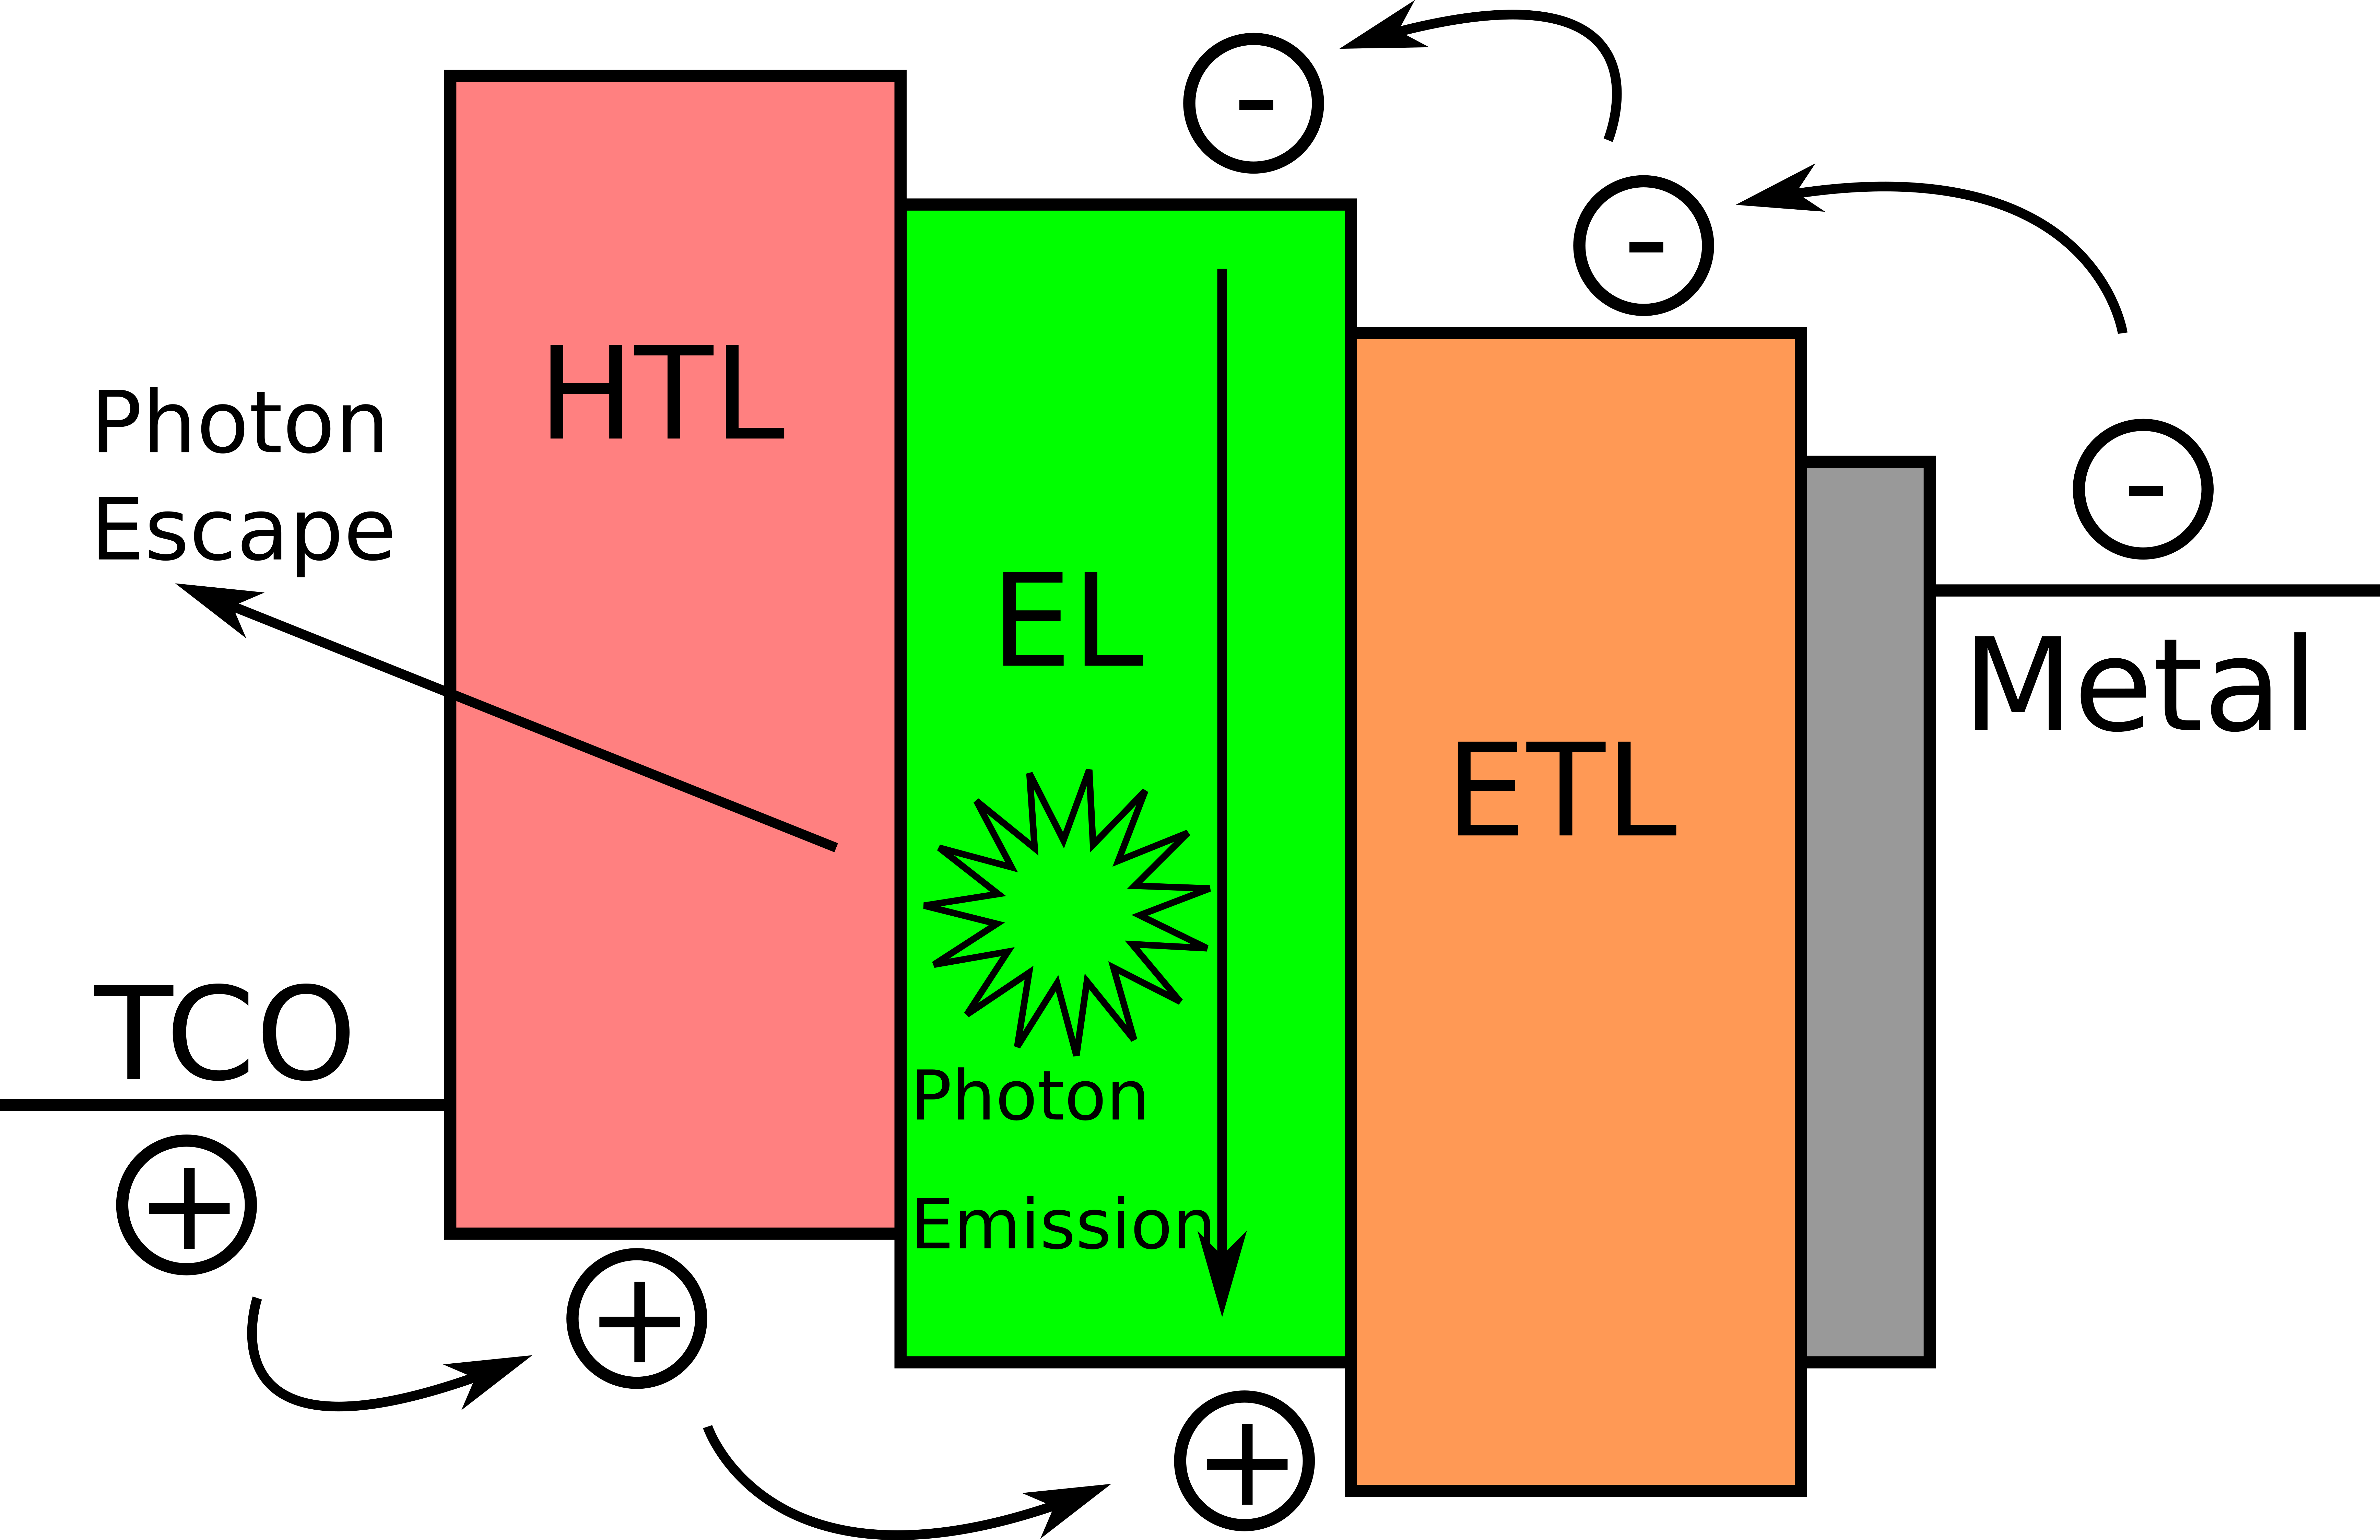
\includegraphics[width=\textwidth]{images/oled_band_diagram.png}
				\end{column}

            \end{columns}

        \end{frame}
        
    \subsection{Waveguides and the Fabry-P\'erot Etalon}
        \begin{frame}
            \frametitle{Waveguides}
        \end{frame}
        \begin{frame}
            \frametitle{The Fabry-P\'erot Etalon}
            \centering
            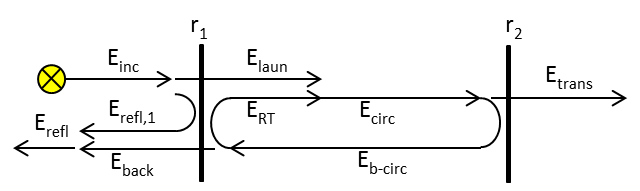
\includegraphics[width=0.75\textwidth]{images/etalon_schematic.png}\\
            $$T(\phi)=\frac{\qty(1-R_1)\qty(1-R_2)}{\qty(1-\sqrt{R_1R_2})^2+4\sqrt{R_1R_2}\sin^2(\phi)}$$
            $$T_{\phi=0}=\frac{\qty(1-R_1)\qty(1-R_2)}{\qty(1-\sqrt{R_1R_2})^2}$$
        \end{frame}
        
    \subsection{Microcavity-confined OLEDs}
        \begin{frame}
            \frametitle{Microcavity-confined OLEDs}
            \begin{columns}
				\begin{column}{0.5\textwidth}
				\end{column}
				\begin{column}{0.5\textwidth}
					\centering
					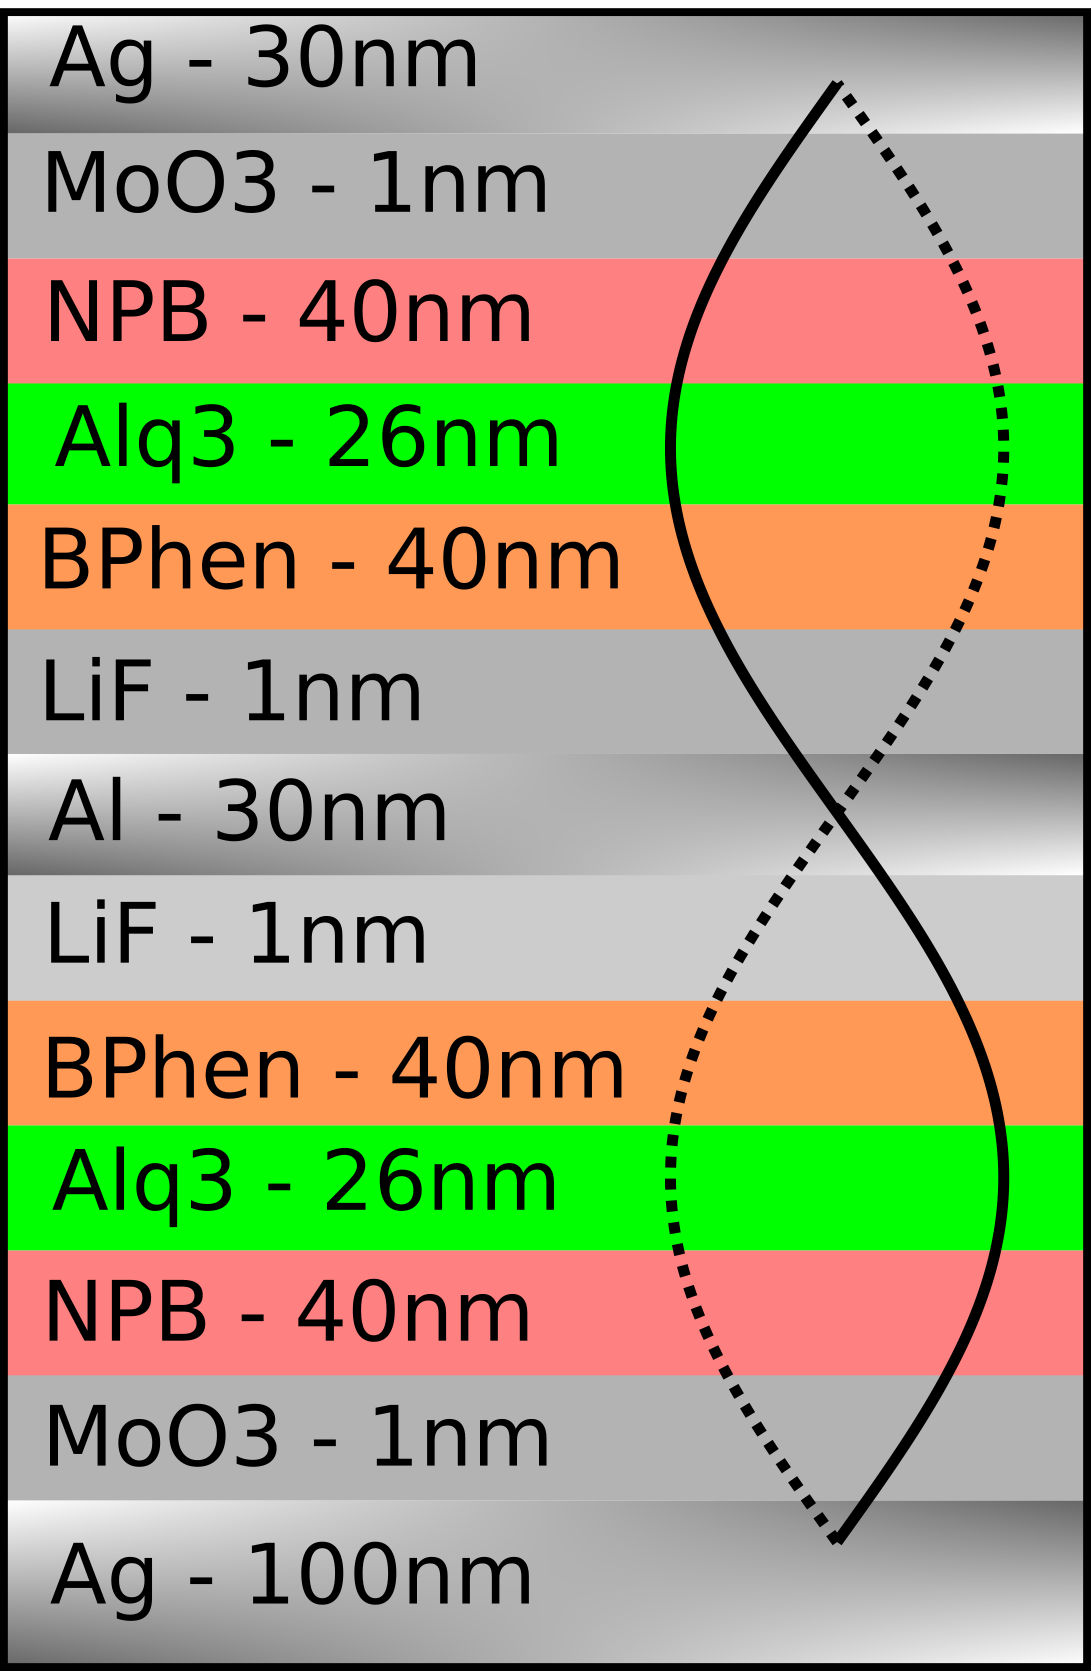
\includegraphics[width=0.8\textwidth]{images/schematic.png}
				\end{column}
            \end{columns}

        \end{frame}
        
\section{Experimental Methods}
    \frame{\tableofcontents[currentsection]}
    \subsection{Device Fabrication}
		\begin{frame}
			\frametitle{Device Fabrication}
			\centering
			\includegraphics[width=\textwidth]{images/microcavity_band_diagram.png}
			\vspace{0.5cm}
			\begin{columns}
				\begin{column}{0.3\textwidth}
					\centering
					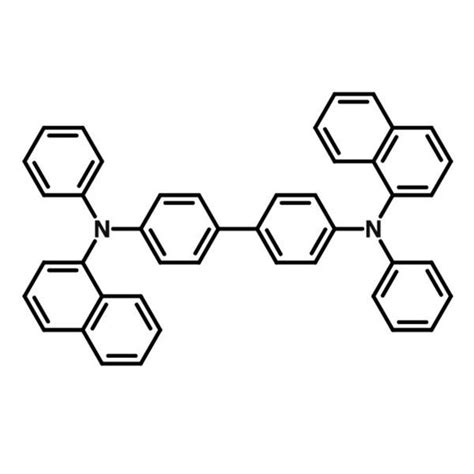
\includegraphics[width=0.8\textwidth]{images/npb_structure.jpg}\\
					\tiny NPB hole transport material
				\end{column}
				\begin{column}{0.3\textwidth}
					\centering
					\includegraphics[width=0.8\textwidth]{images/Alq3_structure.png}\\
					\tiny Alq$_3$ emissive material
				\end{column}
				\begin{column}{0.3\textwidth}
					\centering
					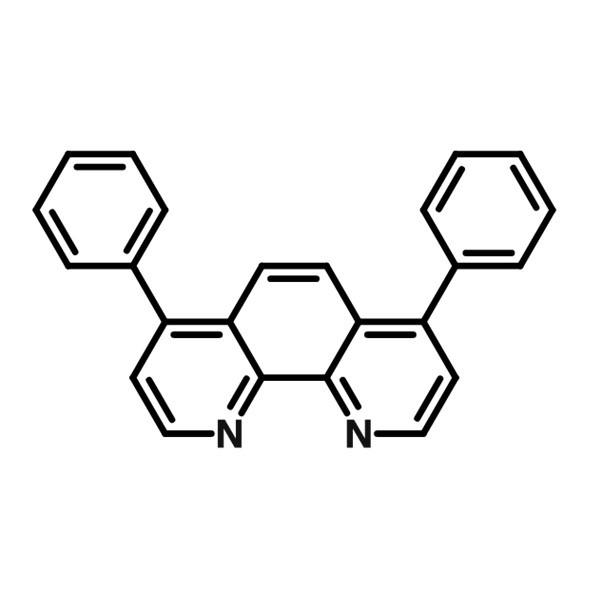
\includegraphics[width=0.8\textwidth]{images/bphen_structure.jpg}\\
					\tiny BPhen electron transport material
				\end{column}
			\end{columns}
		\end{frame}
    
    \subsection{Angle-Resolved Electroluminescence Spectroscopy}
		\begin{frame}
			\frametitle{Angle-Resolved Electroluminescence Spectroscopy (ARES)}
		\end{frame}
    
\section{Results}
    \frame{\tableofcontents[currentsection]}
    
    \subsection{Single Cavity Devices}
        \begin{frame}
            \frametitle{Single Cavity Devices}
            \begin{columns}
                \begin{column}{0.4\textwidth}
					Test
                \end{column}
                \begin{column}{0.6\textwidth}
					\centering
					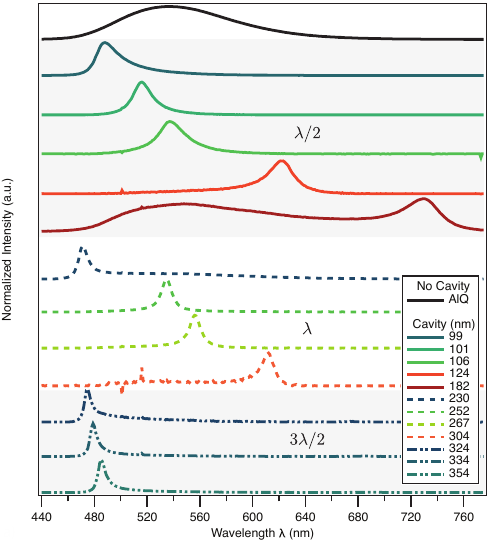
\includegraphics[width=\textwidth]{images/n1_spectra.png}
                \end{column}
            \end{columns}
        \end{frame}
        
        \begin{frame}
            \frametitle{Peak Emission Wavelength}
            \begin{columns}
                \begin{column}{0.4\textwidth}
					\centering
					$$\lambda_0=\frac{2nd}{q}$$
					$n\ \rightarrow$ index of refraction\\
					$d\ \rightarrow$ cavity thickness\\
					$q\ \rightarrow$ resonant mode\\
					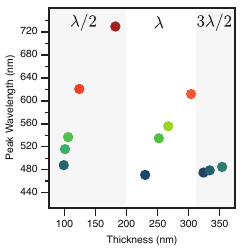
\includegraphics[width=\textwidth]{images/n1_peak_emission.png}
                \end{column}
                \begin{column}{0.6\textwidth}
					\centering
					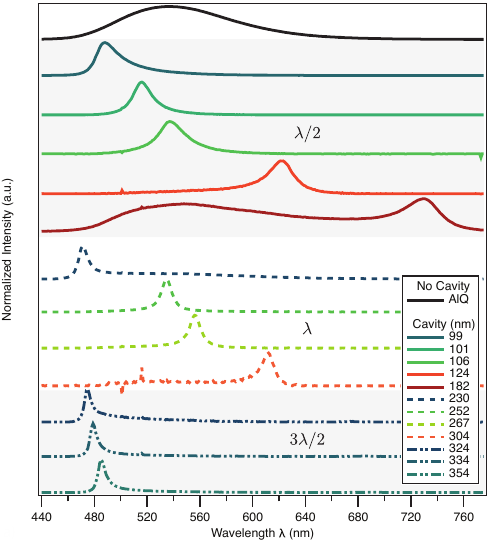
\includegraphics[width=\textwidth]{images/n1_spectra.png}
                \end{column}
            \end{columns}
        \end{frame}
        
        \begin{frame}
            \frametitle{Band Narrowing}
            \begin{columns}
                \begin{column}{0.4\textwidth}
					\centering
					$$Q=\frac{2nd}{\lambda_0}\qty{\frac{1-\sqrt{R_1R_2}}{\pi\qty(R_1R_2)^{1/4}}}$$
					$$Q=q\qty{\frac{1-\sqrt{R_1R_2}}{\pi\qty(R_1R_2)^{1/4}}}$$
					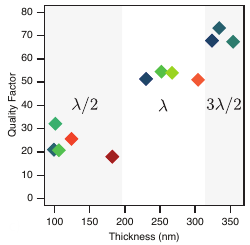
\includegraphics[width=\textwidth]{images/n1_quality_factor.png}
                \end{column}
                \begin{column}{0.6\textwidth}
					\centering
					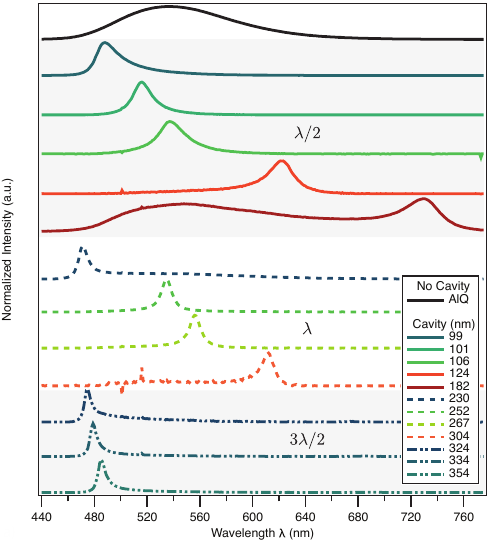
\includegraphics[width=\textwidth]{images/n1_spectra.png}
                \end{column}
            \end{columns}
        \end{frame}
        
        \begin{frame}
            \frametitle{Effect of Bottom Electrode Material}
            \begin{columns}
				\begin{column}{0.5\textwidth}
					\centering
					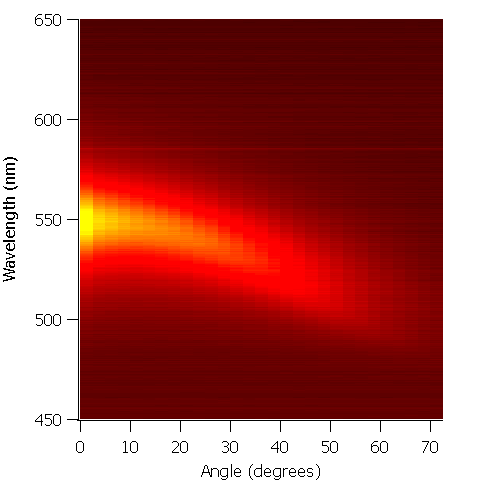
\includegraphics[width=\textwidth]{images/n1_ag_top_heatmap.png}
					Aluminum bottom electrode
				\end{column}
				\begin{column}{0.5\textwidth}
					\centering
					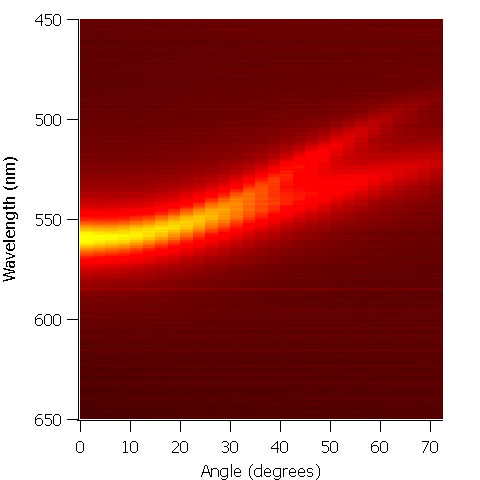
\includegraphics[width=\textwidth]{images/n1_al_top_heatmap.png}
					Silver bottom electrode
				\end{column}


            \end{columns}

        \end{frame}
        
    \subsection{Multi-cavity Devices}
        \begin{frame}
            \frametitle{Multi-cavity Devices}
        \end{frame}
        
        \begin{frame}
            \frametitle{Behavior at Large Angles}
            \begin{columns}
				\begin{column}{0.5\textwidth}
					\centering
					N=2 cavities\\
					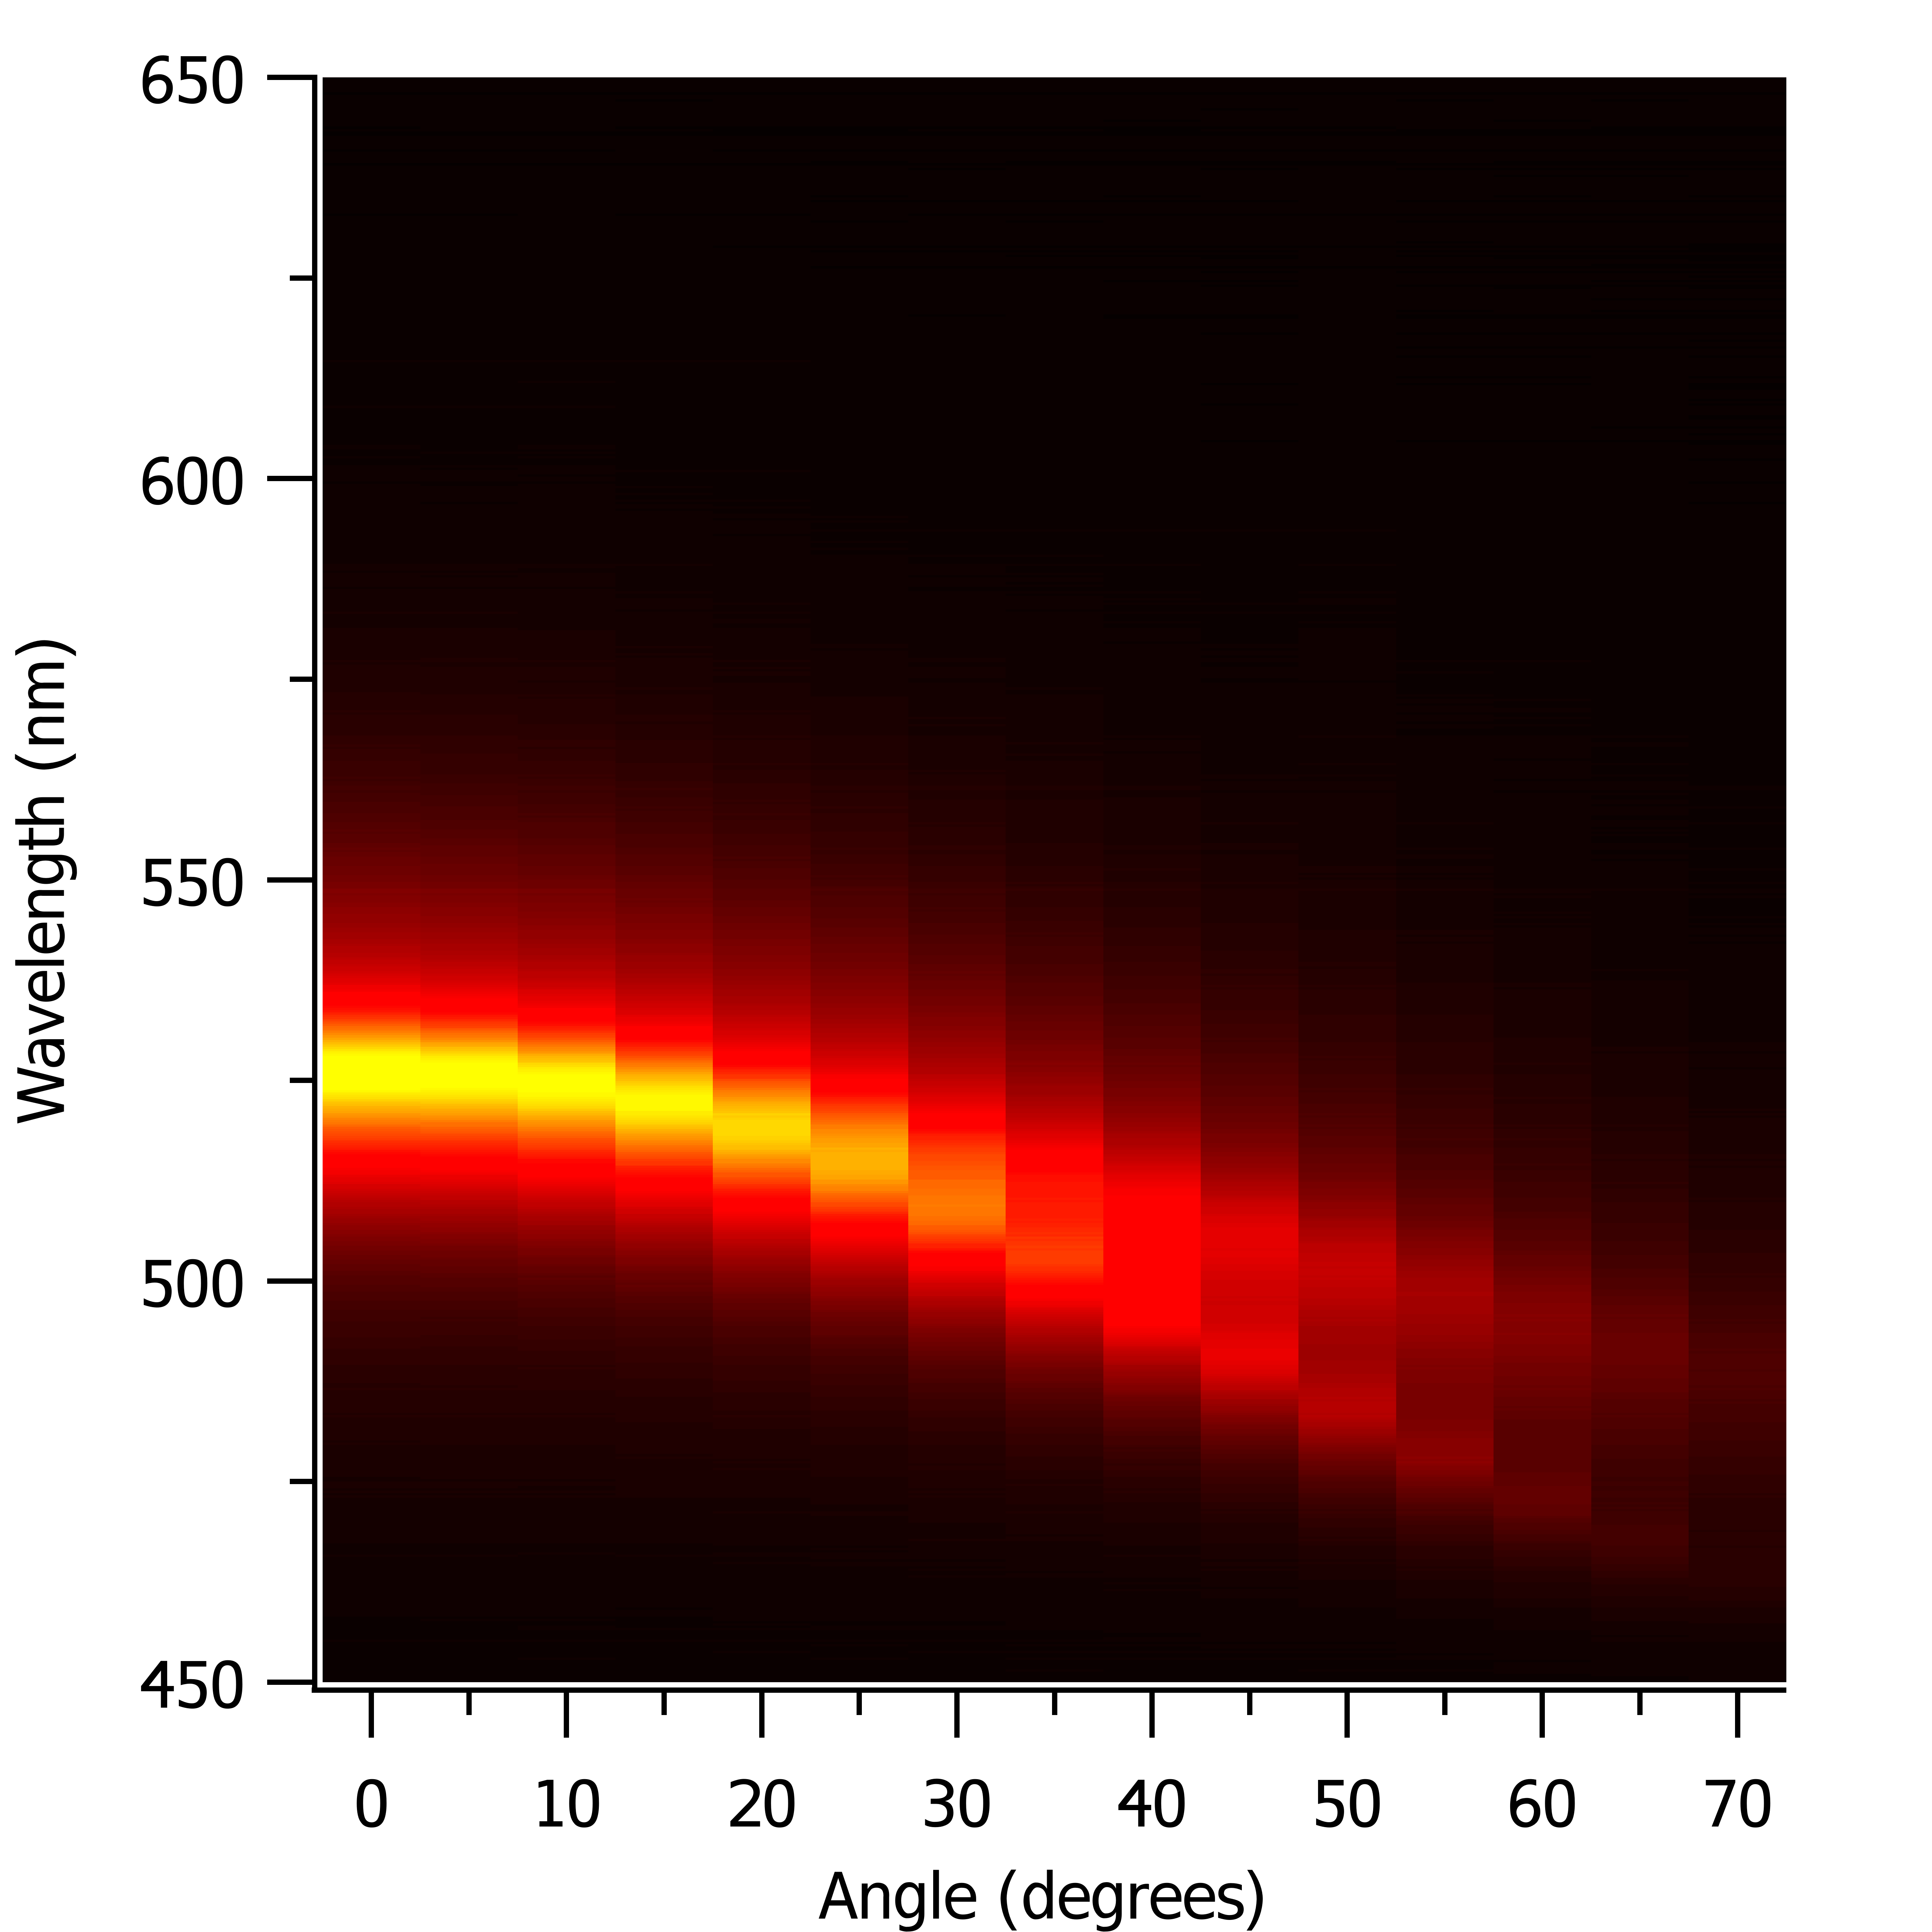
\includegraphics[width=0.7\textwidth]{images/n2_heatmap.png}\\
					N=4 cavities\\
					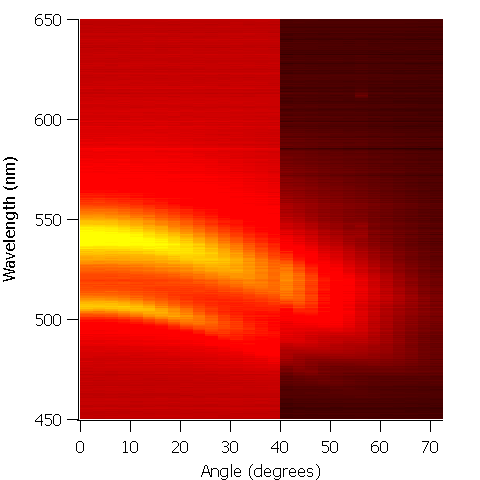
\includegraphics[width=0.7\textwidth]{images/n4_heatmap.png}
				\end{column}
				\begin{column}{0.5\textwidth}
					\centering
					N=3 cavities\\
					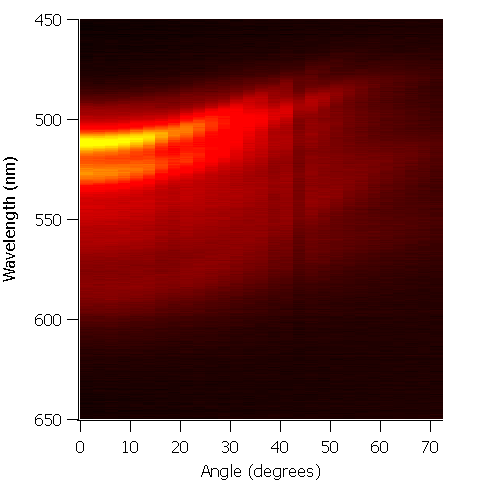
\includegraphics[width=0.7\textwidth]{images/n3_heatmap.png}\\
					N=5 cavities\\
					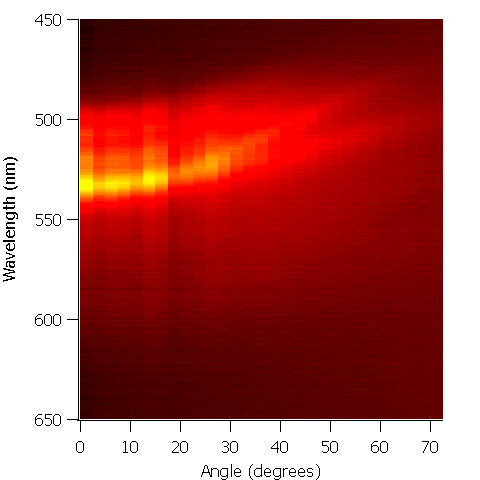
\includegraphics[width=0.7\textwidth]{images/n5_heatmap.png}
				\end{column}
            \end{columns}
        \end{frame}
        
        \begin{frame}
            \frametitle{Number and Bandwidth of Resonant Modes}
            \begin{columns}
				\begin{column}{0.5\textwidth}
					\centering
					N=2 cavities\\
					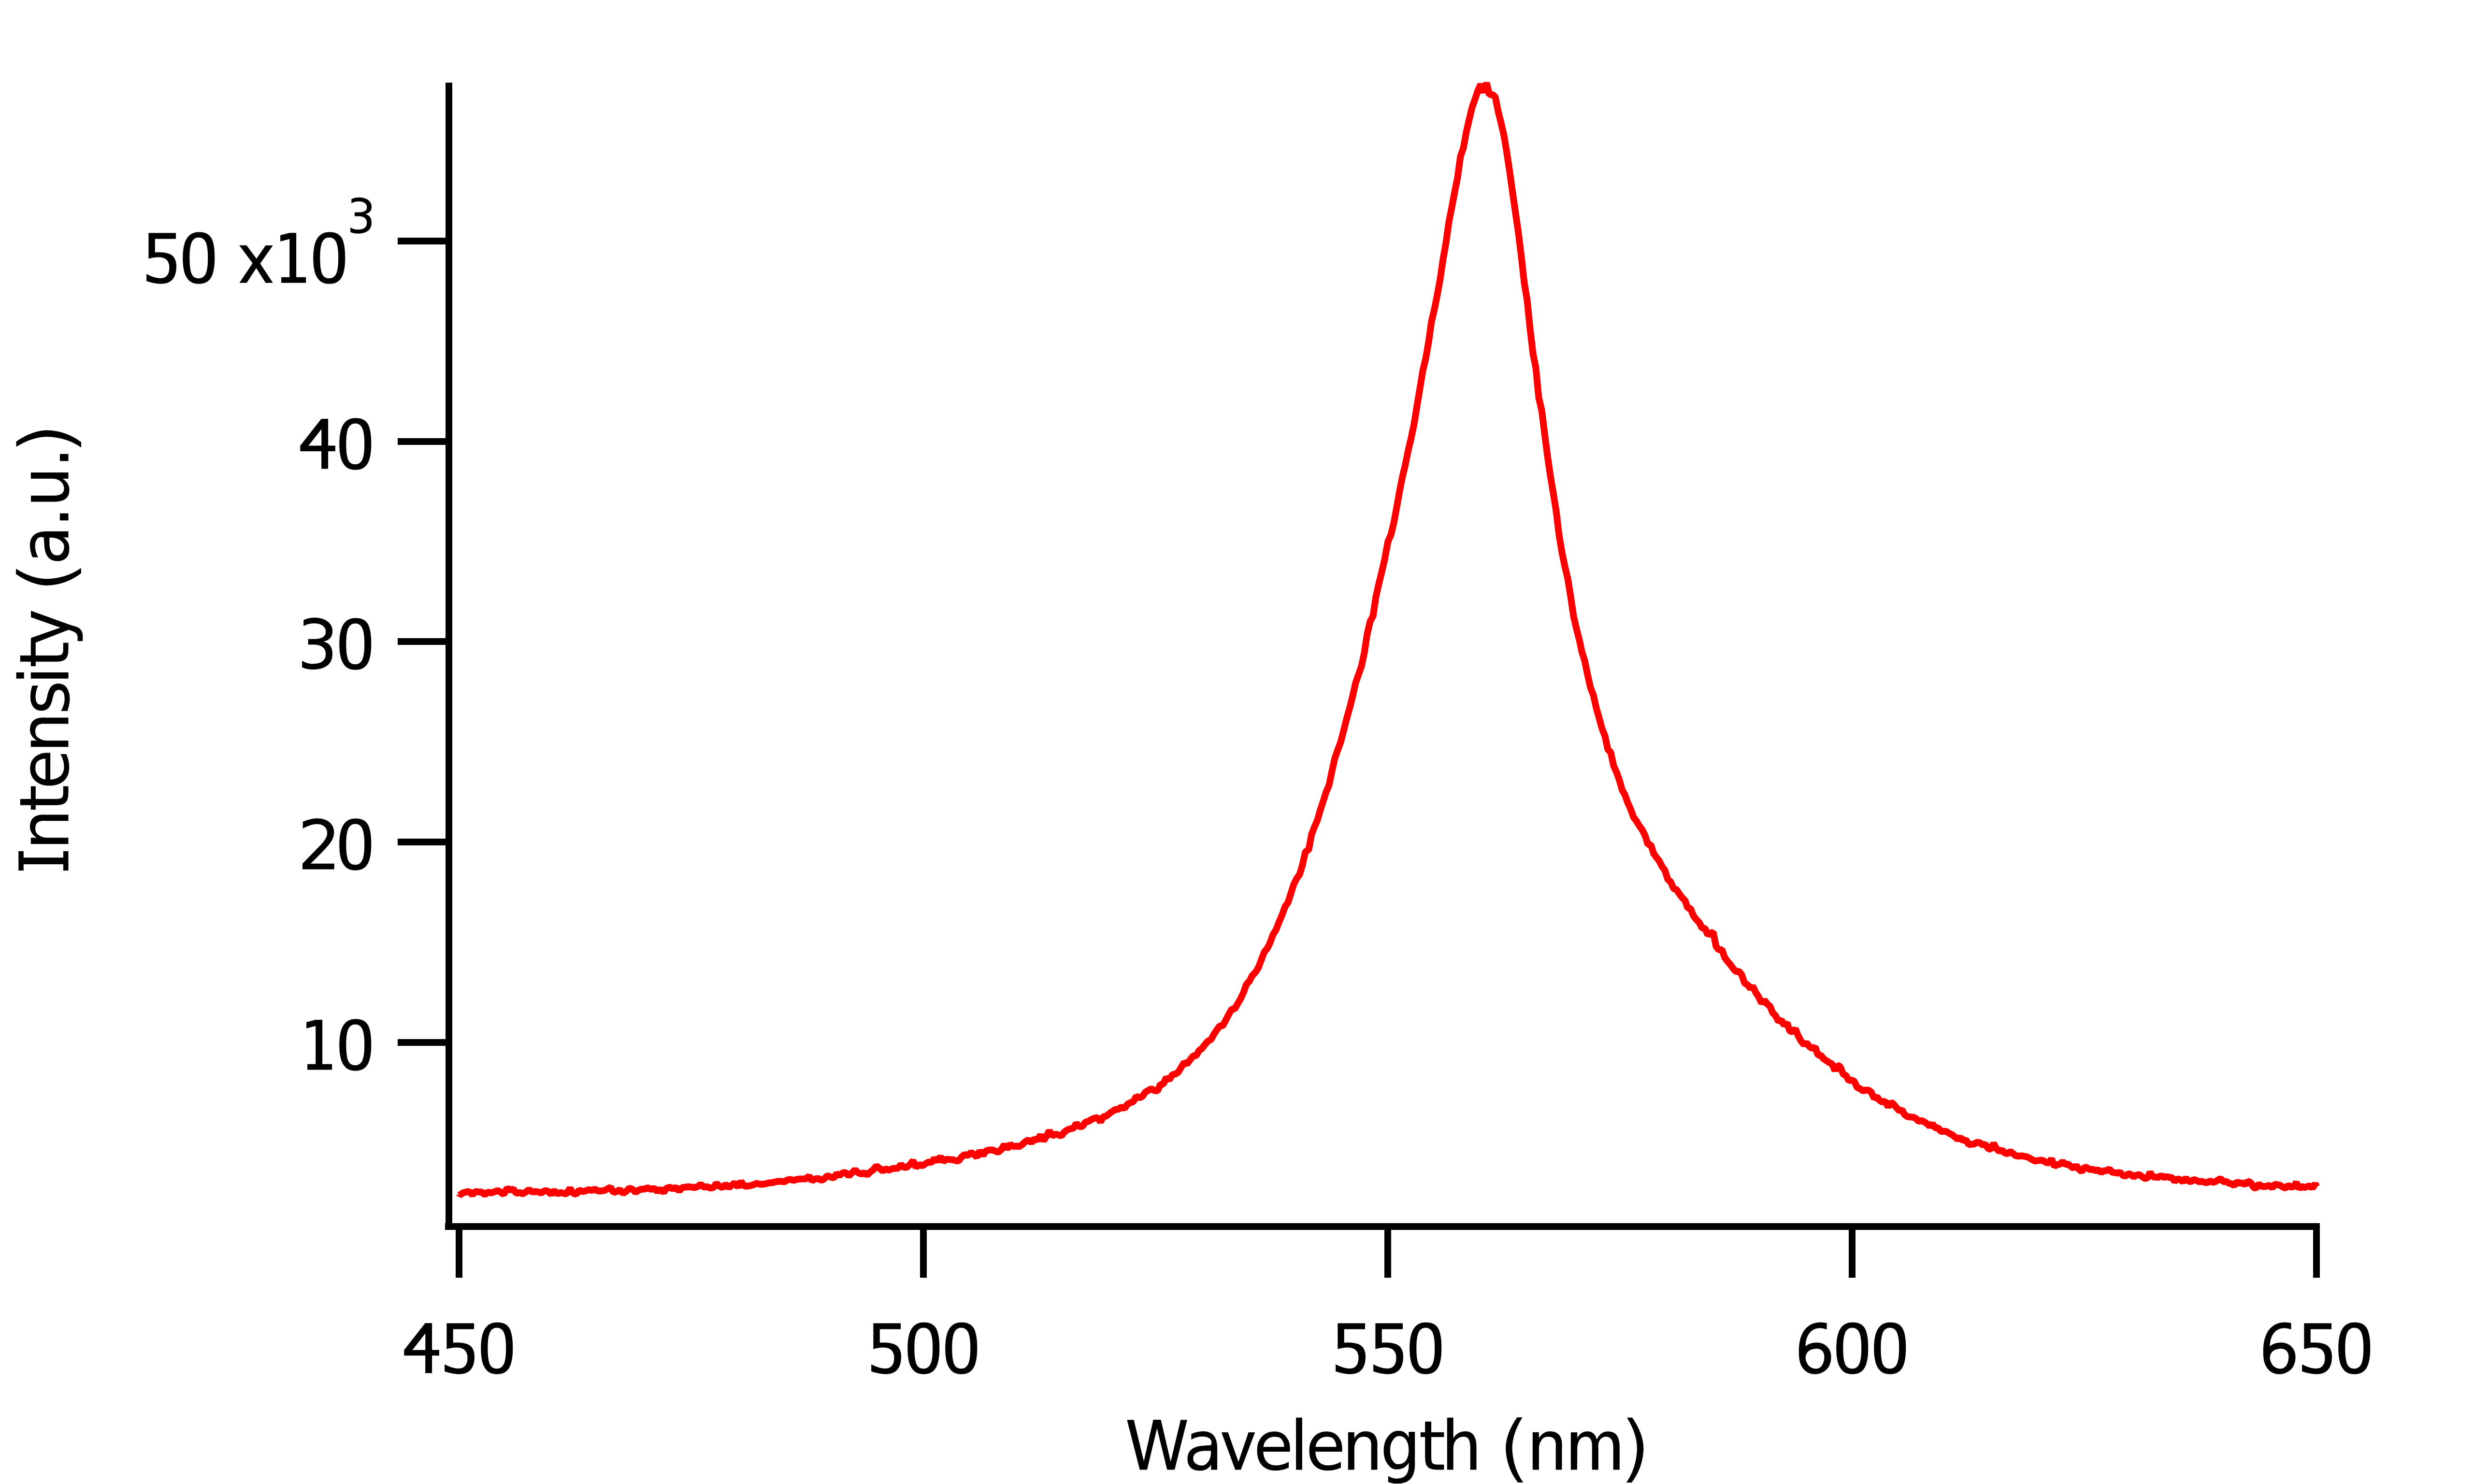
\includegraphics[width=\textwidth]{images/n2_fe.png}\\
					N=4 cavities\\
					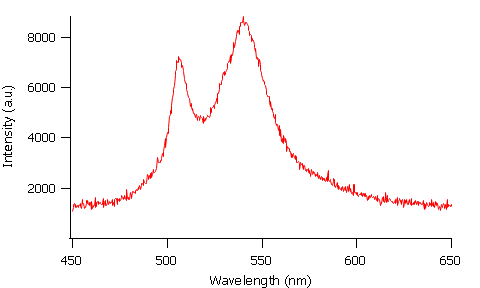
\includegraphics[width=\textwidth]{images/n4_fe.png}
				\end{column}
				\begin{column}{0.5\textwidth}
					\centering
					N=3 cavities\\
					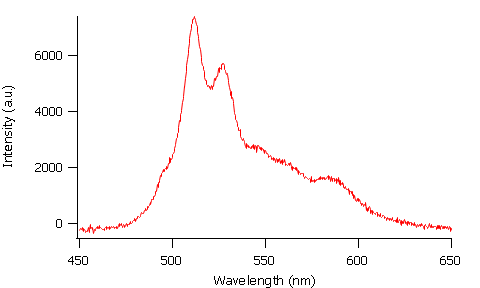
\includegraphics[width=\textwidth]{images/n3_fe.png}\\
					N=5 cavities\\
					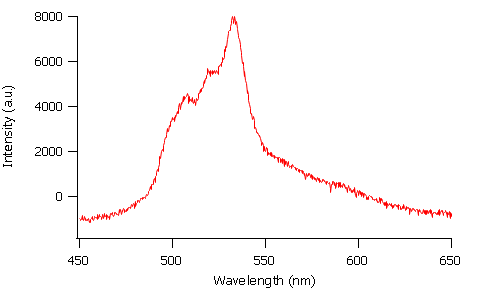
\includegraphics[width=\textwidth]{images/n5_fe.png}
				\end{column}
            \end{columns}
        \end{frame}
        
\section{Conclusions}
    \frame{\tableofcontents[currentsection]}
    \begin{frame}
        \frametitle{Conclusions and Future Work}
    \end{frame}
    
    \begin{frame}
        \frametitle{References}
    \end{frame}
    
    \begin{frame}
        \frametitle{Acknowledgements}
    \end{frame}
    
    \begin{frame}
        \frametitle{Questions?}
        \centering
        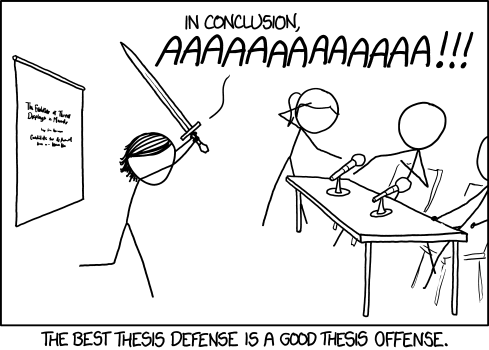
\includegraphics[width=0.75\textwidth]{images/xkcd.png}\\
        \tiny https://xkcd.com/1403/
    \end{frame}
    
\end{document}
